\noindent\begin{tikzpicture}[remember picture]

\begin{pgfonlayer}{front}

\coordinate (titulo_c) at (0,0);

\ifdefined\titulo
\node [name=titulo_t,
  anchor=north west,
  fill=white,
  text = black,
  align=center %,
  %text width=.8\paperwidth
  %minimum width=\paperwidth
  ,opacity=0
] at (titulo_c) {
  \ifdefined\mobile
    \begin{varwidth}{\textwidth}\Large{\textsc{\titulo}}\end{varwidth}
  \else
    \begin{varwidth}{\textwidth}\huge{\textsc{\titulo}}\end{varwidth}
  \fi
};
\coordinate [below=0.01\paperheight] (autor_c) at (titulo_t.south west);
\else
\coordinate (titulo_t) at (titulo_c);
\coordinate [below=0.01\paperheight] (autor_c) at (titulo_t);
\fi

\ifdefined\autor
\node [name=autor_t,
  ,anchor=north west
  ,fill=white
  ,text = black
  ,align=center
  ,opacity=0
] at (autor_c) {
  \ifdefined\mobile
    \begin{varwidth}{\textwidth}\large{\textsc{\autor}}\end{varwidth}};
\else
\begin{varwidth}{\textwidth}\Large{Escrito por \textsc{\autor}}\end{varwidth}};
\fi
\coordinate [below=0.01\paperheight] (tradutor_c) at (autor_t.south west);
\else
\coordinate (autor_t) at (autor_c);
\coordinate [below=0.01\paperheight] (tradutor_c) at (autor_t);
\fi

\ifdefined\tradutor
\node [name=tradutor_t,
  ,anchor=north west
  ,fill=white
  ,text = black
  ,align=center
  ,opacity=0
] at (tradutor_c) {
  \ifdefined\mobile
    \begin{varwidth}{\textwidth}{Tradução: \textsc{\tradutor}}\end{varwidth}};
\else
\begin{varwidth}{\textwidth}\large{Traduzido por \textsc{\tradutor}}\end{varwidth}};
\fi
\coordinate [below=0.01\paperheight] (poster_c) at (tradutor_t.south west);
\else
\coordinate (tradutor_t) at (tradutor_c);
\coordinate [below=0.01\paperheight] (poster_c) at (tradutor_t);
\fi

\ifdefined\URL
\ifdefined\CriadorDestePDF
\ifdefined\mobile
\def \poster {<\URL>, por \textsc{\CriadorDestePDF}\newline\today}
\else
\def \poster {Discussão em <\URL>, por \textsc{\CriadorDestePDF} em \today}
\fi
\else
\ifdefined\mobile
\def \poster {<\URL>\newline\today}
\else
\def \poster {Discussão em <\URL>, \today}
\fi
\fi
\else
\ifdefined\CriadorDestePDF
\ifdefined\mobile
\def \poster {Arquivo por \textsc{\CriadorDestePDF}\newline\today}
\else
\def \poster {Arquivo gerado por \textsc{\CriadorDestePDF} em \today}
\fi
\else
\ifdefined\mobile
\def \poster {\today}
\else
\def \poster {Gerado em \today}
\fi
\fi
\fi

\node [name=poster_t,
  ,anchor=north west
  ,fill=white
  ,text = black
  ,align=center
  ,opacity=0
] at (poster_c) {
  \begin{varwidth}{\textwidth}\poster\end{varwidth}};


\coordinate [below=0.07\paperheight] (branco_c) at (poster_t.south west);


\end{pgfonlayer}
\end{tikzpicture}

\noindent\begin{tikzpicture}[remember picture,overlay]

\coordinate (nw) at (current page.north west);
\ifdefined\capa
\noindent\begin{pgfonlayer}{bg}    % select the background layer
\noindent\node[inner sep=0, anchor=north west,name=capa] at (current page.north west) {
  \ifdefined\mobile
    \noindent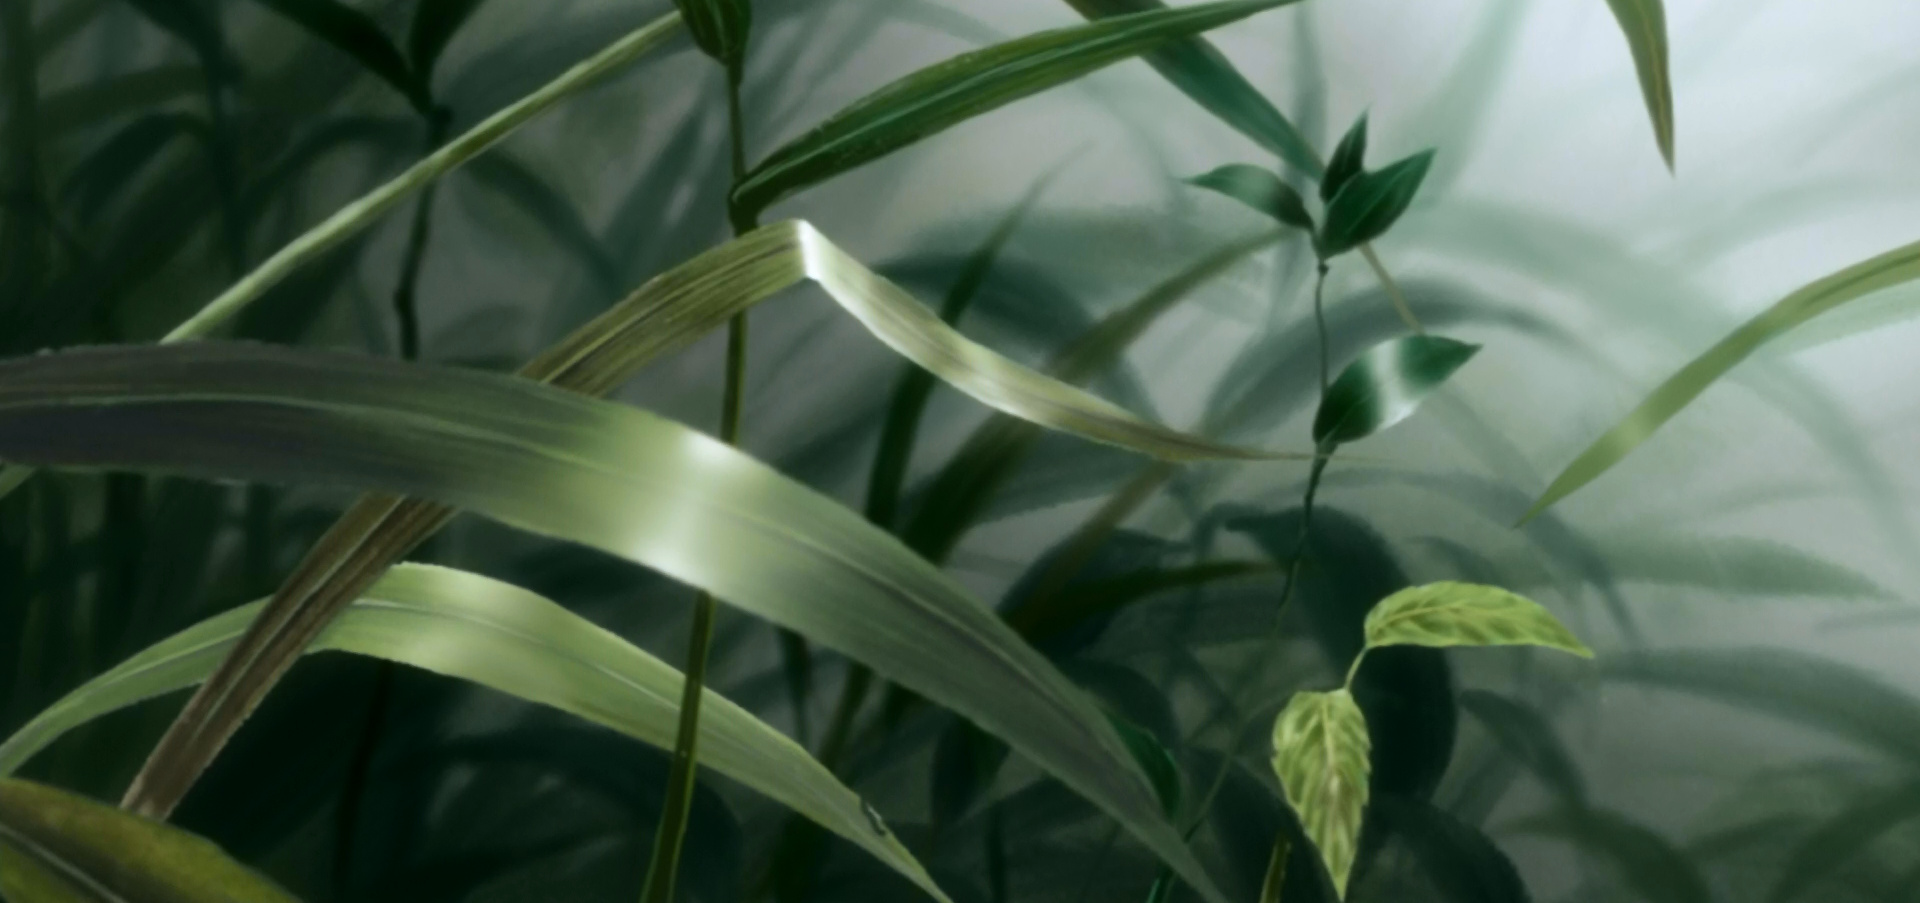
\includegraphics[min width=\paperwidth,min height=\paperheight,keepaspectratio]{\capa}
  \else
    \noindent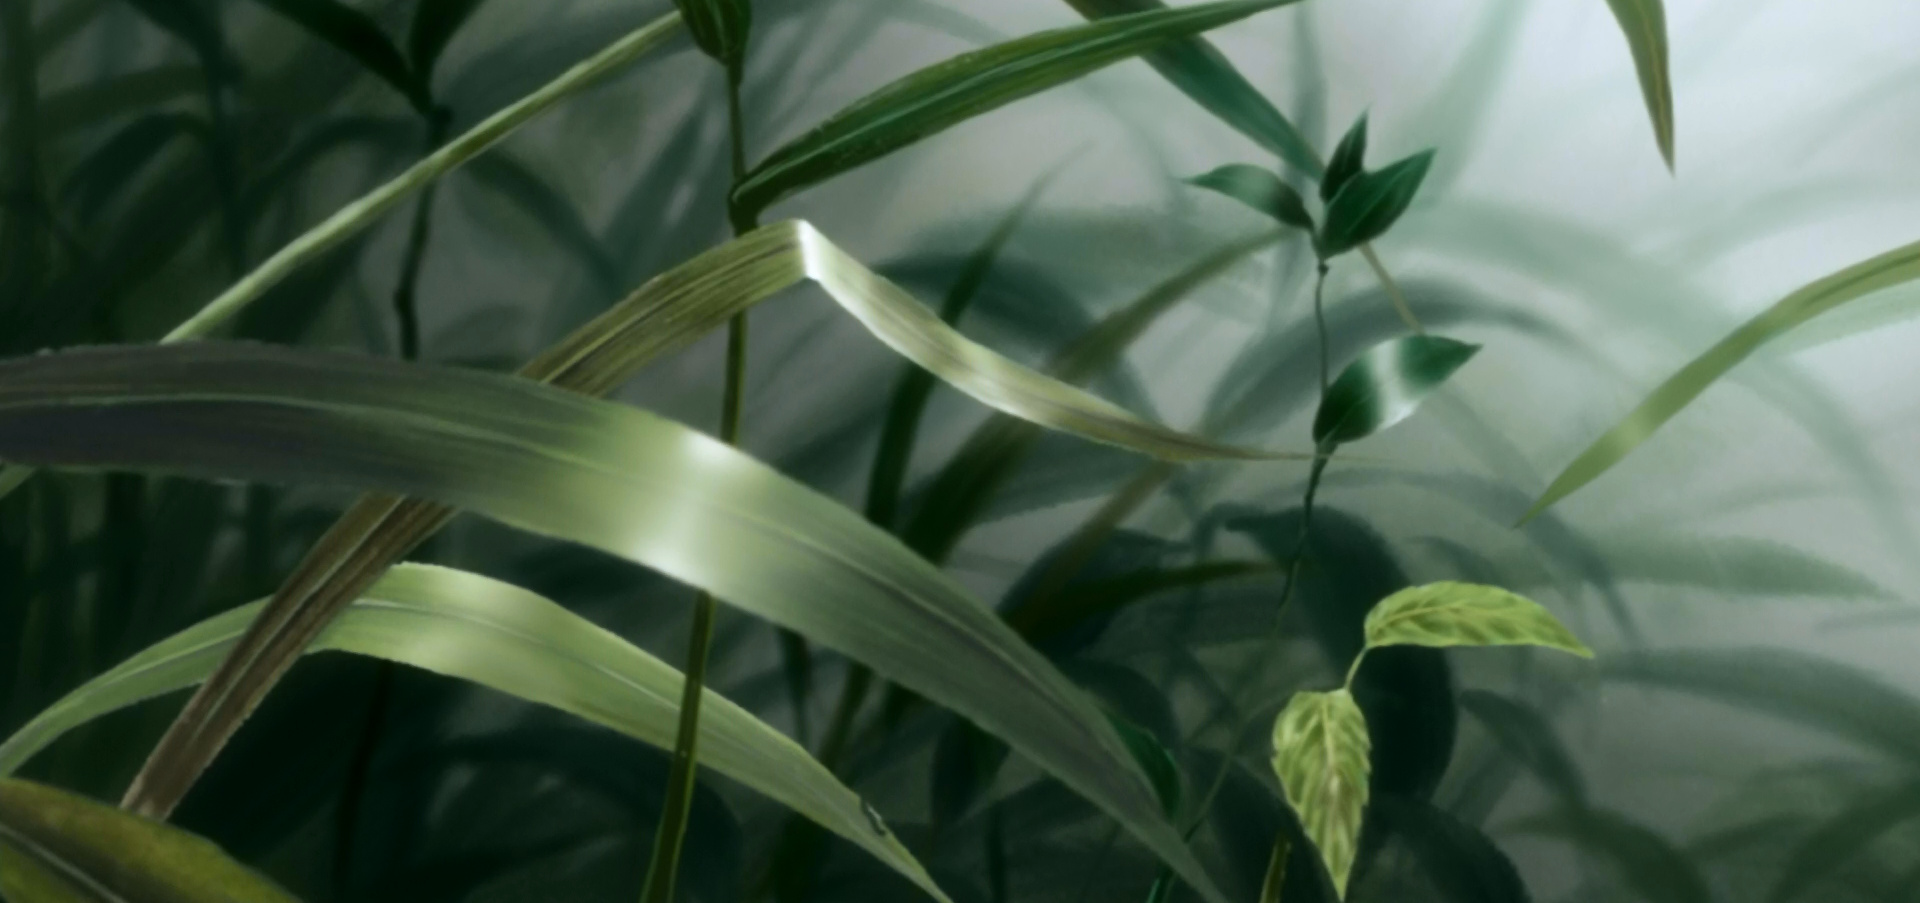
\includegraphics[width=\paperwidth,keepaspectratio]{\capa}
  \fi
};

\ifdefined\mobile
\else
\fill [anchor=west, fill=white] (-11,0) rectangle (current page.south east);
\fi


\end{pgfonlayer}
\fi


\begin{pgfonlayer}{front}    % select the background layer
%\coordinate [ajuste] (nome) at (lugar)


  \coordinate (zero) at (0,0);
  \coordinate (titulo_c2) at ($ (titulo_t.north west) + (zero) - (titulo_c) + (0,1) $);


  \ifdefined\mobile
  \def \tituloL {.5cm}
  \def \tituloU {-.5cm}
  \else
  \def \tituloL {.95in}
  \def \tituloU {-.052\paperheight}
  \fi

  \ifdefined\titulo
  \node [name=titulo_t2,
  anchor=north west,
  fill=white,
  text = black,
  %align=center %,
  %text width=.8\paperwidth
  %minimum width=\paperwidth
  ,fill opacity=0.8
  ,text opacity=1
  %,left=-6.1cm
  ] at ($ (nw) + (\tituloL,\tituloU) $) {
    \ifdefined\mobile
      \begin{varwidth}{\textwidth}\Large{\textsc{\titulo}}\end{varwidth}
    \else
      \begin{varwidth}{\textwidth}\huge{\textsc{\titulo}}\end{varwidth}
    \fi
  };

\coordinate [below=0.01\paperheight] (autor_c2) at (titulo_t2.south west);
\else
\coordinate (titulo_t2) at (titulo_c2);
\coordinate [below=0.01\paperheight] (autor_c2) at (titulo_t2);
\fi

\ifdefined\autor
\node [name=autor_t2,
  ,anchor=north west
  ,fill=white
  ,text = black
  ,align=center
  ,fill opacity=0.8
  ,text opacity=1
] at (autor_c2) {
  \ifdefined\mobile
    \begin{varwidth}{\textwidth}\large{\textsc{\autor}}\end{varwidth}};
\else
\begin{varwidth}{\textwidth}\Large{Escrito por \textsc{\autor}}\end{varwidth}};
\fi
\coordinate [below=0.01\paperheight] (tradutor_c2) at (autor_t2.south west);
\else
\coordinate (autor_t2) at (autor_c2);
\coordinate [below=0.01\paperheight] (tradutor_c2) at (autor_t2);
\fi

\ifdefined\tradutor
\node [name=tradutor_t2,
  ,anchor=north west
  ,fill=white
  ,text = black
  ,align=center
  ,fill opacity=0.8
  ,text opacity=1
] at (tradutor_c2) {
  \ifdefined\mobile
    \begin{varwidth}{\textwidth}{Tradução: \textsc{\tradutor}}\end{varwidth}};
\else
\begin{varwidth}{\textwidth}\large{Traduzido por \textsc{\tradutor}}\end{varwidth}};
\fi
\coordinate [below=0.01\paperheight] (poster_c2) at (tradutor_t2.south west);
\else
\coordinate (tradutor_t2) at (tradutor_c2);
\coordinate [below=0.01\paperheight] (poster_c2) at (tradutor_t2);
\fi

\ifdefined\URL
\ifdefined\CriadorDestePDF
\ifdefined\mobile
\def \poster {<\URL>, por \textsc{\CriadorDestePDF}\newline\today}
\else
\def \poster {Discussão em <\URL>, por \textsc{\CriadorDestePDF} em \today}
\fi
\else
\ifdefined\mobile
\def \poster {<\URL>\newline\today}
\else
\def \poster {Discussão em <\URL>, \today}
\fi
\fi
\else
\ifdefined\CriadorDestePDF
\ifdefined\mobile
\def \poster {Arquivo por \textsc{\CriadorDestePDF}\newline\today}
\else
\def \poster {Arquivo gerado por \textsc{\CriadorDestePDF} em \today}
\fi
\else
\ifdefined\mobile
\def \poster {\today}
\else
\def \poster {Gerado em \today}
\fi
\fi
\fi

\node [name=poster_t2,
  ,anchor=north west
  ,fill=white
  ,text = black
  ,align=center
  ,fill opacity=0.8
  ,text opacity=1
] at (poster_c2) {
  \begin{varwidth}{.6945\paperwidth}{\poster}\end{varwidth}};



\end{pgfonlayer}

\end{tikzpicture}

